\subsection{Gameplay Loop}
Der primäre \textit{Gameplay Loop} besteht darin, die Bienenkolonie am Leben zu halten. Nach Spielbeginn wird der Spieler mit den gegebenen Arbeitsbienen und der Königin auf sich alleine gestellt. Der Spieler sollte damit anfangen, etwas Nektar und Pollen zu sammeln, um diese dann zu Bienenwachs zu verarbeiten und einen Stock zu bauen. Innerhalb dieses Stocks sollte die Königin beginnen, Drohnen heranzuziehen, mit welchen man wiederum neue Arbeiterinnen und/oder eine neue Königin heranziehen kann. Das Ziel besteht darin, das Überleben der Kolonie möglichst lange zu sichern. Die Herausforderung besteht darin, dass die Winter schwer sind und mit der Zeit auch immer schwerer werden. Es gilt, die Balance zu finden zwischen Nahrungsbeschaffung, Erweiterung des Stocks und Erzeugung neuer Brut. Zeugt der Spieler zu viel neue Bienen, kippt das Gleichgewicht und die Kolonie stirbt an einem Mangel an Nahrung. Das grobe Konzept des Gameplay Loops ist in \autoref{image:gameplayloop} veranschaulicht.

\begin{figure}
    \begin{center}
        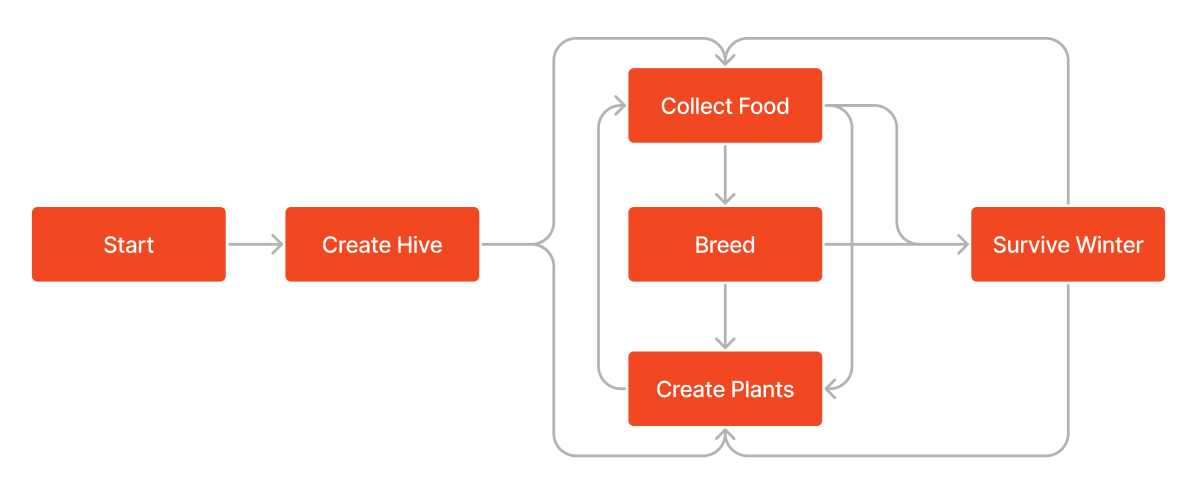
\includegraphics[width=300px]{0.bilder/gameplayloop.PNG}
    \end{center}
    \caption{Grobe Skizze des Gameplay Loops} \label{image:gameplayloop}
\end{figure}